% %%%%%%%%%%%%%%%%%%%%%%%%%%%%%%%%%%%%%%%%%%%%%%%%%%%%%%%%%%%%%%%%%%%%%%%%%
% %%% INICIO INPUT SEMANA 2 %%%
% (Corta desde aquí hasta la marca de "FIN INPUT SEMANA 2" 
% para pegarlo en "semana2.tex")
% %%%%%%%%%%%%%%%%%%%%%%%%%%%%%%%%%%%%%%%%%%%%%%%%%%%%%%%%%%%%%%%%%%%%%%%%%

\chapter{Semana 2: Rotaciones en el Círculo y Transitividad}

\section{Rotaciones en $S^1$}

Consideremos el cociente $\mathbb{R}/\mathbb{Z}$, donde $x \sim y \iff x - y \in \mathbb{Z}$. Este espacio puede ser identificado con el intervalo $[0,1)$ o con el círculo unidad $S^1 \subset \mathbb{C}$ mediante la biyección $[x] \mapsto e^{2\pi i x}$.

\begin{definicion}[Rotación en el Círculo]
	Dado un ángulo $\theta \in (0,1)$, definimos la \textbf{rotación de ángulo $\theta$} como la aplicación $R_\theta: \mathbb{R}/\mathbb{Z} \to \mathbb{R}/\mathbb{Z}$ dada por:
	$$R_\theta([x]) = [x + \theta]$$
	En la notación compleja de $S^1$, equivale a $R_\theta(z) = e^{2\pi i \theta} z$.
\end{definicion}

\begin{proposicion}
	Si $\theta \in \mathbb{Q}$, $\theta = p/q$ con $p, q \in \mathbb{Z}$, $q > 0$ y $(p,q)=1$ (fracción irreducible), entonces $R_\theta^q(z) = z, \forall z \in S^1$, y además $R_\theta^j(z) \neq z$ para $j=1,2,\dots,q-1$. Es decir, todos los puntos son periódicos de periodo exactamente $q$.
\end{proposicion}
\begin{proof}
	Tenemos $R_\theta^q(z) = e^{2\pi i \theta q} z = e^{2\pi i (p/q) q} z = e^{2\pi i p} z = z$.
	
	Supongamos que $\exists q_0 \in \{1,2,\dots,q-1\}$ tal que $R_\theta^{q_0}(z) = z$ para algún $z \in S^1$. Por el algoritmo de Euclides para la división: $q = q_0 \tau + r$, con $0 \le r < q_0$. 
	Luego, 
	$$z = R_\theta^q(z) = R_\theta^{q_0 \tau + r}(z) = R_\theta^r(R_\theta^{q_0 \tau}(z)) = R_\theta^r(z)$$
	Esto implica que $z = e^{2\pi i \theta r} z \implies 1 = e^{2\pi i \theta r} \implies \theta r = k \in \mathbb{Z}$. 
	Por tanto, $\theta = k/r = p/q \implies p r = k q$. Como $p$ y $q$ son primos entre sí ($(p,q)=1$), deducimos que $q$ debe dividir a $r$. Sin embargo, sabemos por el algoritmo de Euclides que $r < q_0 < q$, lo cual genera un absurdo, demostrando que $q$ es el menor entero positivo que cumple la condición.
\end{proof}

\begin{observacion}
	Si $\theta \in \mathbb{Q}$, la órbita de cualquier punto es finita y está dada por:
	$$\mathcal{O}_{R_\theta}(z) = \{R_\theta^n(z) : n \in \mathbb{Z}\} = \{z, R_\theta(z), \dots, R_\theta^{q-1}(z)\}$$
\end{observacion}

\begin{proposicion}
	Si $\theta \notin \mathbb{Q}$, la rotación $R_\theta$ no admite puntos periódicos.
\end{proposicion}

\begin{proof}
	Supongamos por contradicción que existe un punto periódico. Es decir, existen $[x] \in \mathbb{R}/\mathbb{Z}$ y $n \in \mathbb{N}$ tales que $R_\theta^n([x]) = [x]$. Por la definición de la rotación, esto implica que $[x + n\theta] = [x]$.
	Por lo tanto, la diferencia debe ser un número entero: $(x + n\theta) - x = k$ para algún $k \in \mathbb{Z}$. Esto implica que $n\theta = k \implies \theta = k/n$. Como $k, n \in \mathbb{Z}$ y $n \neq 0$, deducimos que $\theta \in \mathbb{Q}$, lo cual contradice la hipótesis de que $\theta$ es irracional.
\end{proof}

\begin{teorema}
	Si $\theta \notin \mathbb{Q}$, entonces para todo $z \in S^1$, la órbita futura es densa. Es decir: $\overline{\mathcal{O}_{R_\theta}^+(z)} = S^1$.
\end{teorema}

\begin{proof}
	Supongamos por el absurdo que $\overline{\mathcal{O}_{R_\theta}^+(z)} \neq S^1$. Denotemos $A = \overline{\mathcal{O}_{R_\theta}^+(z)}$. Como $A$ es cerrado propio, su complemento $A^c$ es abierto y no vacío, por lo que puede expresarse como la unión disjunta de sus componentes conexas, que son arcos abiertos en el círculo: $A^c = \bigcup (a_i, b_i)$.
	Dado que $A$ es un conjunto invariante bajo isometría (rotación), la distancia entre puntos se preserva. Es claro que $R_\theta(A) = A$. Tomando complementos, deducimos que $R_\theta(A^c) = A^c$.
	
	Como $R_\theta$ es un homeomorfismo, mapea componentes conexas en componentes conexas. Así, la imagen de un arco componente $(a, b) \subset A^c$ es otro arco $R_\theta(a, b) = (a+\theta, b+\theta) \subset A^c$. Al ser componentes conexas del mismo conjunto, solo hay dos opciones: o son exactamente el mismo arco, o son disjuntos.
	Si $R_\theta(a, b) = (a, b)$, entonces los extremos deben fijarse (bajo rotación completa, lo cual es imposible pues $\theta \notin \mathbb{Q}$). Por tanto, los arcos $R_\theta^n(a, b)$ son todos disjuntos para $n \in \mathbb{N}$.
	Como $R_\theta$ preserva la longitud, todos estos infinitos arcos disjuntos tienen la misma longitud $L = b-a > 0$. Sin embargo, la suma de las longitudes de infinitos arcos disjuntos daría infinito, lo cual es absurdo ya que todos están contenidos en $S^1$ que tiene longitud $2\pi$. Por lo tanto, $A$ debe ser todo $S^1$.
\end{proof}

\section{Conjugación Topológica}

\begin{definicion}[Conjugación Topológica]
	Sean $M, N$ espacios topológicos y $f: M \to M$, $g: N \to N$ aplicaciones continuas. Decimos que $f$ y $g$ son \textbf{topológicamente conjugadas} si existe un homeomorfismo $h: M \to N$ tal que $h \circ f = g \circ h$.
\end{definicion}

\begin{ejemplo}
	Considere la función tienda $f(x) = \begin{cases} 2x & 0 \le x < 1/2 \\ 2-2x & 1/2 \le x \le 1 \end{cases}$ en $[0,1]$ y la función logística $g(x) = 4x(1-x)$ en $[0,1]$. Muestre que $f$ y $g$ son topológicamente conjugadas y construya el homeomorfismo $h$.
\end{ejemplo}
\begin{proof}[Solución]
	Consideremos la función $h: [0,1] \to [0,1]$ dada por $h(x) = \sin^2\left(\frac{\pi x}{2}\right)$. 
	Primero verificamos que es biyectiva y continua: es continua al ser composición de seno, cuadrado y una función lineal. Su derivada es $h'(x) = \pi \sin(\frac{\pi x}{2}) \cos(\frac{\pi x}{2}) = \frac{\pi}{2} \sin(\pi x) > 0$ en $(0,1)$, por lo que es estrictamente creciente. Como $h(0)=0$ y $h(1)=1$, es una biyección continua de $[0,1]$ sobre sí mismo. 
	Por el teorema clásico de topología general, como $h$ es una biyección continua desde un espacio compacto ($[0,1]$) hacia un espacio de Hausdorff, esto garantiza que $h$ es un homeomorfismo.
	
	\begin{figure}[htbp]
		\centering
		\begin{minipage}{0.31\textwidth}
			\centering
			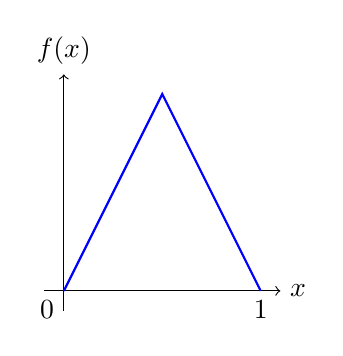
\begin{tikzpicture}[scale=2.5]
				\draw[->] (-0.1,0) -- (1.1,0) node[right] {$x$};
				\draw[->] (0,-0.1) -- (0,1.1) node[above] {$f(x)$};
				\draw[thick, blue] (0,0) -- (0.5,1) -- (1,0);
				\node[below left] at (0,0) {$0$};
				\node[below] at (1,0) {$1$};
			\end{tikzpicture}
			\caption*{Mapa Tienda $f(x)$}
		\end{minipage}\hfill
		\begin{minipage}{0.31\textwidth}
			\centering
			\begin{tikzpicture}[scale=2.5]
				\draw[->] (-0.1,0) -- (1.1,0) node[right] {$x$};
				\draw[->] (0,-0.1) -- (0,1.1) node[above] {$h(x)$};
				\draw[domain=0:1, smooth, variable=\x, purple, thick] plot ({\x}, {sin(\x*90)*sin(\x*90)});
				\node[below left] at (0,0) {$0$};
				\node[below] at (1,0) {$1$};
			\end{tikzpicture}
			\caption*{Conjugación $h(x)$}
		\end{minipage}\hfill
		\begin{minipage}{0.31\textwidth}
			\centering
			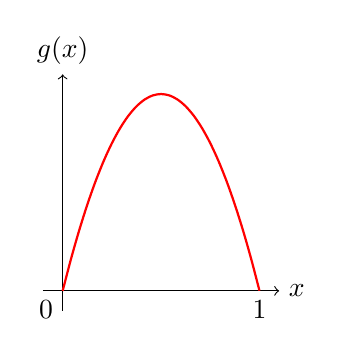
\begin{tikzpicture}[scale=2.5]
				\draw[->] (-0.1,0) -- (1.1,0) node[right] {$x$};
				\draw[->] (0,-0.1) -- (0,1.1) node[above] {$g(x)$};
				\draw[domain=0:1, smooth, variable=\x, red, thick] plot ({\x}, {4*\x*(1-\x)});
				\node[below left] at (0,0) {$0$};
				\node[below] at (1,0) {$1$};
			\end{tikzpicture}
			\caption*{Mapa Logístico $g(x)$}
		\end{minipage}
		\caption{Gráficas de la función tienda $f$, el homeomorfismo $h$ y la función logística $g$ que ilustran la conjugación topológica.}
		\label{fig:conj_tienda_logistica}
	\end{figure}
	
	Ahora verificamos la relación de conjugación $h(f(x)) = g(h(x))$:
	Por un lado, $g(h(x)) = 4\sin^2(\frac{\pi x}{2})\left[1 - \sin^2(\frac{\pi x}{2})\right] = 4\sin^2(\frac{\pi x}{2})\cos^2(\frac{\pi x}{2}) = \left(2\sin(\frac{\pi x}{2})\cos(\frac{\pi x}{2})\right)^2 = \sin^2(\pi x)$.
	
	Por otro lado, evaluamos $h(f(x))$ en ambos tramos de $f$:
	Si $x \in [0, 1/2)$, $h(f(x)) = \sin^2(\frac{\pi(2x)}{2}) = \sin^2(\pi x)$.
	Si $x \in [1/2, 1]$, $h(f(x)) = \sin^2(\frac{\pi(2-2x)}{2}) = \sin^2(\pi - \pi x)$. Por identidades trigonométricas, $\sin(\pi - \alpha) = \sin(\alpha)$, así que $\sin^2(\pi - \pi x) = \sin^2(\pi x)$.
	En ambos casos $h(f(x)) = \sin^2(\pi x) = g(h(x))$. Por lo tanto, son conjugadas.
\end{proof}

\begin{ejemplo}
	Considere $f: \mathbb{R} \to \mathbb{R}$ dada por $f(x) = \frac{1}{2}x$ y $g: \mathbb{R} \to \mathbb{R}$ dada por $g(x) = \frac{1}{3}x$. Muestre que $f$ y $g$ son topológicamente conjugadas, y construya el homeomorfismo $h: \mathbb{R} \to \mathbb{R}$ tal que $h \circ f = g \circ h$.
\end{ejemplo}
\begin{proof}[Solución]
	Necesitamos algún $h: \mathbb{R} \to \mathbb{R}$ tal que $h(x/2) = \frac{1}{3}h(x) \implies 3h(x/2) = h(x)$.
	Supongamos una función de la forma $h(x) = x^\alpha$. Sustituyendo, $3(x/2)^\alpha = x^\alpha \implies 3 = 2^\alpha \implies \alpha = \log_2 3$.
	
	Definimos entonces la función $h: \mathbb{R} \to \mathbb{R}$ considerando los signos:
	$$ h(x) = \begin{cases} 
		x^{\log_2 3} & : x \ge 0 \\ 
		-(-x)^{\log_2 3} & : x < 0 
	\end{cases} $$
	Claramente conjuga la dinámica. Además, al igual que sus funciones generadoras en sus respectivos intervalos (e.g. $[0, +\infty)$ y $(-\infty, 0)$), es claro que $h$ es biyectiva y continua.
\end{proof}

\begin{teorema}
	Sean $M, N$ espacios topológicos y $f: M \to M, g: N \to N$ aplicaciones continuas topológicamente conjugadas vía el homeomorfismo $h: M \to N$. Entonces:
	\begin{enumerate}[1)]
		\item $p \in M$ es punto periódico de $f$ de periodo "$n$" $\iff h(p)$ es un punto periódico de $g$ de periodo "$n$".
		\item $h(\mathcal{O}_f^+(x)) = \mathcal{O}_g^+(h(x)), \forall x \in M$ y $h(\mathcal{O}_f(x)) = \mathcal{O}_g(h(x))$ cuando $f$ y $g$ son homeomorfismos.
		\item $h(\omega_f(x)) = \omega_g(h(x)), \forall x \in M$ y $h(\alpha_f(x)) = \alpha_g(h(x))$ cuando $f$ y $g$ son homeomorfismos.
		\item $h(\Omega(f)) = \Omega(g)$.
	\end{enumerate}
\end{teorema}

\begin{proof}
	\textbf{1)} $[\Rightarrow]$ Sea $f^n(p)=p$ y $f^j(p) \neq p, \forall j \in \{1,\dots,n-1\}$. Tenemos: $h \circ f = g \circ h \implies h \circ f \circ f = g \circ h \circ f = g \circ g \circ h \implies h \circ f^2 = g^2 \circ h$. Generalizando, obtenemos que $h \circ f^n = g^n \circ h, \forall n \in \mathbb{Z}^+$.
	Luego: $g^n(h(p)) = h(f^n(p)) = h(p)$. 
	Supongamos que $\exists j \in \{1,\dots,n-1\}$ tal que $g^j(h(p)) = h(p) \implies h(f^j(p)) = h(p) \implies f^j(p) = p$, lo cual es absurdo ya que $n$ es el periodo mínimo de $p$. Así, "$n$" es el periodo de $h(p)$ respecto a $g$.
	
	$[\Leftarrow]$ Por hipótesis: $g^n(h(p)) = h(p)$ y $g^j(h(p)) \neq h(p), \forall j \in \{1,\dots,n-1\}$. Luego, $h(f^n(p)) = h(p) \implies f^n(p) = p$. Supongamos que $\exists j \in \{1,\dots,n-1\}$ tal que $f^j(p) = p \implies h(f^j(p)) = h(p) \implies g^j(h(p)) = h(p)$, un absurdo.
	
	\textbf{2)} Sea $y \in h(\mathcal{O}_f^+(x)) \iff \exists n \in \mathbb{N} / y = h(f^n(x)) \iff \exists n \in \mathbb{N} / y = g^n(h(x)) \iff y \in \mathcal{O}_g^+(h(x))$. Si $f$ y $g$ son homeomorfismos, la demostración para la órbita total es idéntica solo que usamos $\exists n \in \mathbb{Z} / y = h(f^n(x))$.
	
	\textbf{3)} Sea $y \in h(\omega_f(x)) \iff \exists (n_k) \subseteq \mathbb{Z}^+ \land z \in M$ tales que $f^{n_k}(x) \to z \land y = h(z) \iff$ [como $h$ es homeomorfismo] $\exists (n_k) \subseteq \mathbb{Z}^+ / h(f^{n_k}(x)) \to h(z) = y \iff g^{n_k}(h(x)) \to y \iff y \in \omega_g(h(x))$.
	
	\textbf{4)} Sea $y \in h(\Omega(f)) \implies \exists z \in \Omega(f) / h(z) = y$. Sea $V_y$ una vecindad de $y$, entonces $h^{-1}(V_y)$ es un conjunto abierto en $M$.
	Por definición de $\Omega(f)$, $\exists n \in \mathbb{Z}^+ / f^n(h^{-1}(V_y)) \cap h^{-1}(V_y) \neq \emptyset \implies \exists n \in \mathbb{Z}^+ / h(f^n(h^{-1}(V_y))) \cap h(h^{-1}(V_y)) \neq \emptyset \implies g^n(V_y) \cap V_y \neq \emptyset \implies y \in \Omega(g)$. La vuelta es completamente análoga.
\end{proof}

\begin{corolario}
	Sean $R_{r/s}$ y $R_{p/q}$ rotaciones racionales con $r,s,p,q \in \mathbb{Z} \land s,q > 0$ y fracciones irreducibles $(r,s)=1, (p,q)=1$. Entonces: 
	$$R_{r/s} \text{ y } R_{p/q} \text{ son topológicamente conjugadas} \implies s = q$$
\end{corolario}
\begin{proof}
	Sea $x \in S^1$. La cardinalidad de su órbita será exactamente el denominador del ángulo irreducible, es decir, $\text{card}(\mathcal{O}_{R_{r/s}}^+(x)) = s$. 
	Como $h$ es una función biyectiva, preserva la cantidad de elementos, lo que implica que $\text{card}(h(\mathcal{O}_{R_{r/s}}^+(x))) = s$.
	Por conjugación, esto debe ser igual a la cardinalidad de la órbita de $h(x)$ bajo la otra rotación: $\text{card}(\mathcal{O}_{R_{p/q}}^+(h(x))) = q$. Por consiguiente, se concluye que $s = q$.
\end{proof}

\begin{ejercicio}
	Mostrar que: $R_\theta$ y $R_\alpha$ son topológicamente conjugados $\iff \alpha \pm \theta \in \mathbb{Z}$.
\end{ejercicio}

\begin{ejercicio}
	Considere $f: S^1 \to S^1$, definida por $z \mapsto f(z) = z^2$.
	\begin{enumerate}[a)]
		\item Halle $\text{Per}_n(f) = \{z \in S^1 : f^n(z) = z\}$.
		\item Muestre que $\overline{\text{Per}(f)} = S^1$.
	\end{enumerate}
\end{ejercicio}
\begin{proof}[Solución]
	\textbf{a)} Para $n \in \mathbb{N} \land z \in \text{Per}_n(f) \implies f^n(z) = z^{2^n} = z \implies z^{2^n} - z = 0 \implies z(z^{2^n-1} - 1) = 0$.
	De aquí obtenemos $z=0 \lor z$ es una de las $2^n-1$ raíces de la unidad. Como estamos operando en el círculo unidad ($z \in S^1$), descartamos $z=0$. 
	Por tanto, $z = e^{2\pi i \frac{k}{2^n-1}} = \cos\left(2\pi \frac{k}{2^n-1}\right) + i\sin\left(2\pi \frac{k}{2^n-1}\right)$ para $0 \le k < 2^n-1$.
	
	\textbf{b)} Sabemos que las $N$ raíces de la unidad dividen al círculo uniformemente en $N$ partes de igual longitud ($L = 2\pi/N$). Sea un punto cualquiera $z = e^{2\pi i x} \in S^1$.
	Consideramos la biyección $h: [0,1) \to S^1, x \mapsto h(x) = e^{2\pi i x}$. 
	Sea $A$ un conjunto abierto que contiene a $z \implies h^{-1}(A)$ es un abierto que contiene a $x$. Luego existe un $\epsilon > 0 / V_\epsilon(x) \subseteq h^{-1}(A)$. 
	Sea $N \in \mathbb{N}$ un entero suficientemente grande tal que $1/N < \epsilon$ (conceptualmente este $N$ representará los valores $2^n-1$ para $n$ grandes). 
	
	Si $x = j/N$ para algún $j \in \{0, \dots, N-1\} \implies z = e^{2\pi i j/N} \implies z \in \text{Per}_N(f)$, por lo que la vecindad automáticamente lo contiene.
	Si $x \neq j/N, \forall j \in \{0, \dots, N-1\}$, partimos el intervalo $[0,1)$ en $N$ partes iguales. Entonces $x$ pertenece a algún subintervalo, lo que implica que su distancia a alguno de los extremos $j_0/N$ es estrictamente menor a la longitud de la partición: $|x - j_0/N| < 1/N < \epsilon$ para algún $j_0 \in \{0, \dots, N-1\}$.
	Esto asegura que $j_0/N \in V_\epsilon(x)$. Luego, al mapear de regreso, $y = h(j_0/N) \in A$, donde $y$ es evidentemente una raíz de la unidad $y \in \text{Per}_N(f)$. Esto demuestra que cualquier abierto interseca a los puntos periódicos, garantizando la densidad $\overline{\text{Per}(f)} = S^1$.
\end{proof}

\section{Sistemas Dinámicos Topológicamente Transitivos y Mixing}

\begin{definicion}[Topológicamente Transitivo]
	Sea $X$ un espacio topológico. Decimos que $f: X \to X$ es \textbf{topológicamente transitiva} si existe un $x \in X$ tal que su órbita futura es densa, es decir, $\overline{\mathcal{O}^+(x)} = X$.
\end{definicion}

\begin{ejemplo}
	$R_\theta: S^1 \to S^1$ donde $\theta \in \mathbb{R} \setminus \mathbb{Q}$ es topológicamente transitivo, pues $\overline{\mathcal{O}_{R_\theta}^+(z)} = S^1, \forall z \in S^1$.
\end{ejemplo}

\begin{ejemplo}
	$R_\theta: S^1 \to S^1$ donde $\theta \in \mathbb{Q}$ ($\theta = p/q$) implica que $\overline{\mathcal{O}_{R_\theta}^+(z)} = \{z, R_\theta(z), \dots, R_\theta^{q-1}(z)\} \subsetneq S^1$. Así, una rotación racional no es topológicamente transitiva.
\end{ejemplo}

\begin{teorema}
	Sea $X$ un espacio métrico separable (admite base numerable) y localmente compacto, y $f: X \to X$ continua. La función $f$ es topológicamente transitiva si y solo si para cualquier par de abiertos $U, V \subseteq X$ no vacíos, existe $n \in \mathbb{N}$ tal que $f^n(U) \cap V \neq \emptyset$.
\end{teorema}
\begin{proof}
	$(\Rightarrow)$ Supongamos que $f$ es topológicamente transitiva. Entonces existe $x \in X$ con órbita densa. Sean $U, V$ abiertos no vacíos. Por densidad, la órbita debe visitar ambos abiertos, es decir, existen enteros $j < k$ tales que $f^j(x) \in U$ y $f^k(x) \in V$.
	Aplicando $f^{k-j}$ a $f^j(x)$, obtenemos $f^{k-j}(f^j(x)) = f^k(x) \in V$. Como $f^j(x) \in U$, esto demuestra que $f^{k-j}(U) \cap V \neq \emptyset$, con $n = k-j > 0$.
	
	$(\Leftarrow)$ Asumimos la condición de intersección. Como $X$ es separable, admite una base numerable de abiertos $\{B_i\}_{i \in \mathbb{N}}$. Para cada $B_i$, el conjunto $U_i = \bigcup_{n \ge 0} f^{-n}(B_i)$ es la unión de preimágenes de un abierto, por ende es abierto. Afirmamos que cada $U_i$ es denso en $X$. En efecto, si tomamos cualquier abierto $W \subset X$, por hipótesis existe $n$ tal que $f^n(W) \cap B_i \neq \emptyset \implies W \cap f^{-n}(B_i) \neq \emptyset \implies W \cap U_i \neq \emptyset$, probando la densidad.
	Por el Teorema de Categoría de Baire, en un espacio localmente compacto de Hausdorff, la intersección numerable de abiertos densos sigue siendo un conjunto denso. Sea $x \in \bigcap U_i$. Esto implica que para todo básico $B_i$, $x \in \bigcup f^{-n}(B_i) \implies \exists n \text{ t.q. } f^n(x) \in B_i$. Así, la órbita de $x$ visita todo abierto básico, por lo que es densa y $f$ es topológicamente transitiva.
\end{proof}

\begin{ejercicio}
	Si $f: X \to X$ es topológicamente transitiva y $\varphi: X \to \mathbb{R}$ es continua tal que $\varphi(f(x)) = \varphi(x), \forall x \in X \implies \varphi$ es constante.
\end{ejercicio}
\begin{proof}[Solución]
	Supongamos que $\varphi$ no es constante $\implies \exists x, y \in X$ tales que $\varphi(x) \neq \varphi(y)$. 
	Sin pérdida de generalidad, asumamos que $\varphi(x) > \varphi(y) \implies \exists \alpha \in \mathbb{R}$ tal que $\varphi(x) > \alpha > \varphi(y)$.
	Definimos los conjuntos $U = \{z : \varphi(z) > \alpha\}$ y $V = \{z : \varphi(z) < \alpha\}$. Como $\varphi$ es continua, $U$ y $V$ son abiertos, y por la evaluación anterior, $\neq \emptyset$.
	Luego, como $f$ es topológicamente transitiva $\implies \exists k \in \mathbb{Z}^+ / f^k(U) \cap V \neq \emptyset$.
	Es decir, $\exists z \in V$ tal que $z = f^k(a)$ para algún $a \in U$. 
	Como se nos da que $\varphi(f^n(x)) = \varphi(x), \forall n \in \mathbb{N}$, evaluamos en $a$:
	$$ \varphi(z) = \varphi(f^k(a)) = \varphi(a) $$
	Dado que $z \in V \implies \varphi(z) < \alpha$. Pero como $a \in U \implies \varphi(a) > \alpha$. Por ende, obtenemos la contradicción $\varphi(z) > \alpha$ y $\varphi(z) < \alpha$ simultáneamente ($\rightarrow \leftarrow$).
	Por consiguiente, $\varphi$ debe ser constante.
\end{proof}

\begin{ejercicio}
	Sea $X$ un espacio separable y localmente compacto. Sea $f: X \to X$ continua. Mostrar que $f$ no es topológicamente transitiva $\iff \exists U, V \subset X$ abiertos t.q. $U \cap V = \emptyset$, $f(U) \subset U$ y $f(V) \subset V$.
\end{ejercicio}
\begin{proof}[Solución]
	$(\Leftarrow)$ Sean $U, V \subseteq X$ abiertos tales que $U \cap V = \emptyset$.
	Considerando $U' = \bigcup_{n \in \mathbb{N}} f^n(U)$ y $V' = \bigcup_{n \in \mathbb{N}} f^n(V)$, estos son conjuntos abiertos en $X$.
	Notemos que, como $f(U) \subseteq U$, se cumple por inducción que $f^k(U) \subseteq U$ para todo $k \in \mathbb{N}$. 
	De esto se deduce que:
	$$ f^k(U) \cap V \subseteq U \cap V = \emptyset \implies f^k(U) \cap V = \emptyset $$
	Al existir dos abiertos disjuntos cuya iteración nunca se interseca, se concluye que $f$ no es topológicamente transitiva.
	
	$(\Rightarrow)$ Sea $U_0, V_0 \subseteq X$ abiertos. Por la definición de no ser topológicamente transitiva, $\forall k \in \mathbb{Z}^+$ se cumple que $f^k(U_0) \cap V_0 = \emptyset$.
	Considerando $U = \bigcup_{n \in \mathbb{N}} f^n(U_0) \implies U$ es abierto.
	Además, notemos la invariancia: 
	$$f(U) \subseteq f\left(\bigcup_{n \in \mathbb{N}} f^n(U_0)\right) = \bigcup_{n \in \mathbb{N}} f^{n+1}(U_0) \subseteq U$$
	Sea $V = \text{int}(U^c) \implies$ como $X$ es localmente compacto, $V$ es abierto. Cumpliendo así la construcción de conjuntos invariantes y disjuntos requerida.
\end{proof}

\begin{definicion}[Topológicamente Mixing]
	Sea $X$ un espacio topológico y $f: X \to X$ continua. Decimos que $f$ es \textbf{topológicamente mixing} si para cualquier par de abiertos $U, V \subseteq X$ no vacíos, existe un $N \in \mathbb{N}$ tal que para todo $n \ge N$, $f^n(U) \cap V \neq \emptyset$.
\end{definicion}

\begin{observacion}
	Es claro que Topológicamente Mixing $\implies$ Topológicamente Transitivo, ya que la existencia de un $N$ para todos los $n \ge N$ implica fuertemente la existencia de al menos un $n$. El converso no siempre es cierto (por ejemplo, las rotaciones irracionales son transitivas pero no mixing, ya que los intervalos rotan rígidamente sin dispersarse por todo el espacio).
\end{observacion}

\begin{figure}[htbp]
	\centering
	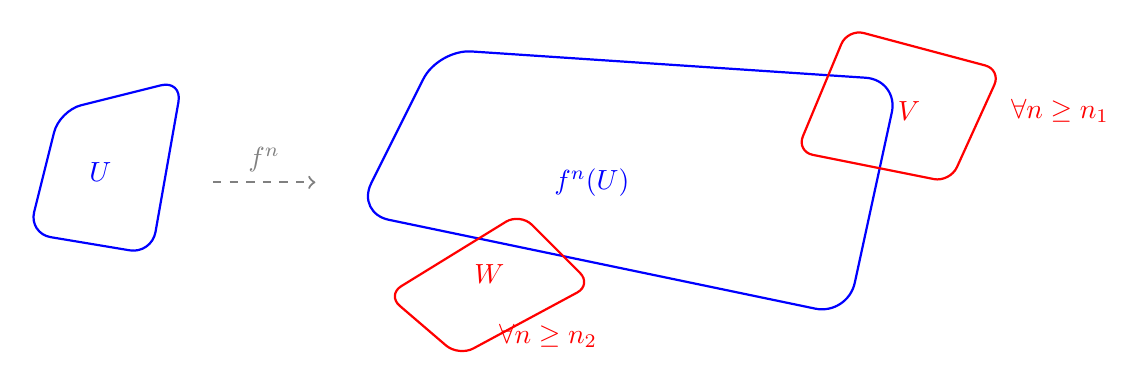
\begin{tikzpicture}[scale=1.3]
		% Conjunto U original
		\draw[blue, thick, rounded corners=8pt] (0,0) -- (0.3,1.2) -- (1.5,1.5) -- (1.2,-0.2) -- cycle;
		\node[blue] at (0.7, 0.6) {$U$};
		
		% Flecha indicando iteración
		\draw[->, thick, gray, dashed] (1.8, 0.5) -- (2.8, 0.5) node[midway, above] {$f^n$};
		
		% f^n(U) expandido
		\draw[blue, thick, rounded corners=12pt] (3.2,0.2) -- (4,1.8) -- (8.5,1.5) -- (8,-0.8) -- cycle;
		\node[blue] at (5.5, 0.5) {$f^n(U)$};
		
		% Conjunto V (intersectado)
		\draw[red, thick, rounded corners=6pt] (7.5, 0.8) -- (8, 2) -- (9.5, 1.6) -- (9, 0.5) -- cycle;
		\node[red] at (8.6, 1.2) {$V$};
		\node[red, right] at (9.5, 1.2) {$\forall n \ge n_1$};
		
		% Conjunto W (intersectado)
		\draw[red, thick, rounded corners=6pt] (3.5, -0.6) -- (4.2, -1.2) -- (5.5, -0.5) -- (4.8, 0.2) -- cycle;
		\node[red] at (4.5, -0.4) {$W$};
		\node[red, right] at (4.5, -1) {$\forall n \ge n_2$};
		
	\end{tikzpicture}
	\caption{Dinámica de un sistema topológicamente mixing. La iteración $f^n(U)$ se expande lo suficiente como para intersecar de forma permanente cualquier otro abierto ($V$, $W$) a partir de cierto umbral temporal.}
	\label{fig:top_mixing_minimalista}
\end{figure}

\begin{ejemplo}
	Consideremos el mapa tienda $f: [0,1] \to [0,1]$ dado por:
	$$ f(x) = \begin{cases} 2x & : 0 \le x \le 1/2 \\ 2-2x & : 1/2 \le x \le 1 \end{cases} $$
	Sabemos que $f([0, 1/2]) = [0,1]$ y $f([1/2, 1]) = [0,1]$.
	De manera más general, las iteraciones sobre los subintervalos diádicos abarcan todo el espacio:
	$$ f^n\left(\left[\frac{i}{2^n}, \frac{i+1}{2^n}\right]\right) = [0,1], \quad \text{para } i=0, \dots, 2^n-1, \forall n \in \mathbb{N} $$
	Sean $U$ y $V \subseteq [0,1]$ abiertos. Existe un $n_0 \in \mathbb{N}$ tal que podemos encajar un subintervalo diádico entero dentro de $U$:
	$$ \exists n_0 \in \mathbb{N} / \left[\frac{i-1}{2^{n_0}}, \frac{i}{2^{n_0}}\right] \subseteq U \text{ para algún } i \in \{1, 2, \dots, 2^{n_0}\} $$
	Aplicando $f^{n_0}$ a ambos lados, obtenemos:
	$$ f^{n_0}\left(\left[\frac{i-1}{2^{n_0}}, \frac{i}{2^{n_0}}\right]\right) \subseteq f^{n_0}(U) \implies [0,1] \subseteq f^{n_0}(U) \implies f^{n_0}(U) = [0,1] $$
	En consecuencia, $f^n(U) = [0,1]$ para todo $n \ge n_0$. Como $V$ es no vacío, $f^n(U) \cap V = [0,1] \cap V = V \neq \emptyset$. Esto demuestra que el mapa tienda es topológicamente mixing.
\end{ejemplo}

\begin{ejercicio}
	Sea $f: S^1 \to S^1$ dada por $f(z) = z^2$. Mostrar que $f$ es topológicamente mixing.
\end{ejercicio}
\begin{proof}[Solución]
	Si utilizamos la representación equivalente en el intervalo $[0,1)$ mediante la identificación del ángulo, la función se comporta como $x \mapsto 2x \pmod 1$.
	Sean $U, V \subseteq S^1$ dos abiertos no vacíos. Como $U$ es un conjunto abierto, este debe contener al menos un pequeño arco continuo de longitud $\epsilon > 0$.
	Cada vez que aplicamos $f$, el ángulo se duplica, por lo que la longitud del arco resultante se multiplica por 2 (considerando solapamientos cuando pasa de $2\pi$). 
	Tras $n$ iteraciones, la imagen $f^n(U)$ abarcará una longitud proyectada de $2^n \epsilon$. 
	Dado que la circunferencia tiene una longitud finita de $2\pi$, podemos elegir un $n_0 \in \mathbb{N}$ lo suficientemente grande tal que:
	$$ 2^{n_0} \epsilon > 2\pi $$
	A partir de este $n_0$, el arco se ha expandido tanto que se enrolla cubriendo todo el círculo, es decir, $f^{n_0}(U) = S^1$. Evidentemente, esta cobertura total se mantendrá para todo $n \ge n_0$, por lo que $f^n(U) = S^1$.
	Finalmente, como $V$ no es vacío, deducimos que:
	$$ f^n(U) \cap V = S^1 \cap V = V \neq \emptyset \quad \forall n \ge n_0 $$
	Concluyendo así que $f(z) = z^2$ es topológicamente mixing.
\end{proof}

\begin{ejercicio}
	Sean $X, Y$ espacios topológicos y $f: X \to X$, $g: Y \to Y$ aplicaciones continuas tales que $f$ y $g$ son topológicamente conjugados vía $h: X \to Y$. Muestre que:
	\begin{enumerate}[1)]
		\item $f$ es topológicamente transitivo $\iff g$ es topológicamente transitivo.
		\item $f$ es topológicamente mixing $\iff g$ es topológicamente mixing.
	\end{enumerate}
\end{ejercicio}
\begin{proof}[Solución]
	Demostraremos la ida ($\Rightarrow$). La vuelta ($\Leftarrow$) es análoga aplicando las mismas propiedades al homeomorfismo inverso $h^{-1}$.
	
	\textbf{1)} Sean $U, V$ abiertos no vacíos en $Y$. Como $h$ es un homeomorfismo, sus preimágenes $h^{-1}(U)$ y $h^{-1}(V)$ son abiertos no vacíos en $X$.
	Dado que $f$ es topológicamente transitiva, existe $n \in \mathbb{N}$ tal que:
	$$ f^n(h^{-1}(U)) \cap h^{-1}(V) \neq \emptyset $$
	Aplicando la función $h$ a toda la intersección (y dado que al ser inyectiva preserva las intersecciones):
	$$ h\left(f^n(h^{-1}(U))\right) \cap h(h^{-1}(V)) \neq \emptyset $$
	Por la definición de conjugación, sabemos que $h \circ f^n = g^n \circ h$. Sustituyendo esto, obtenemos:
	$$ g^n(h(h^{-1}(U))) \cap V \neq \emptyset \implies g^n(U) \cap V \neq \emptyset $$
	Por ende, $g$ también es topológicamente transitiva.
	
	\textbf{2)} Nuevamente, sean $U, V$ abiertos no vacíos en $Y \implies h^{-1}(U), h^{-1}(V)$ son abiertos no vacíos en $X$.
	Como $f$ es topológicamente mixing, existe $n_0 \in \mathbb{N}$ tal que:
	$$ f^n(h^{-1}(U)) \cap h^{-1}(V) \neq \emptyset, \quad \forall n \ge n_0 $$
	Aplicando $h$ a la intersección bajo la misma lógica del punto anterior:
	$$ h\left(f^n(h^{-1}(U))\right) \cap h(h^{-1}(V)) \neq \emptyset, \quad \forall n \ge n_0 $$
	$$ g^n(U) \cap V \neq \emptyset, \quad \forall n \ge n_0 $$
	En consecuencia, $g$ es topológicamente mixing.
\end{proof}

\begin{ejercicio}
	Probar que para un espacio $X$ separable y localmente compacto, la rotación $R_\theta: S^1 \to S^1$ es topológicamente transitiva pero no topológicamente mixing (para $\theta \notin \mathbb{Q}$).
\end{ejercicio}
\begin{proof}[Solución]
	Ya demostramos en semanas anteriores que si el ángulo es irracional, la órbita es densa, garantizando que $R_\theta$ es topológicamente transitiva.
	
	Para probar que no es mixing, vayamos a la representación en el intervalo $[0,1)$, es decir, $R_\theta: [0,1) \to [0,1)$ con $x \mapsto R_\theta(x) = x + \theta \pmod 1$.
	Supongamos por contradicción que es topológicamente mixing $\implies \forall U, V$ abiertos en $[0,1)$, existe $n_0 \in \mathbb{N}$ tal que $R_\theta^n(U) \cap V \neq \emptyset$ para todo $n \ge n_0$.
	
	Vamos a dividir el intervalo $[0,1)$ en $32$ partes iguales. Sea $\varepsilon_0 = 1/32$. Tomemos estos abiertos específicos:
	$$ U = V_{\varepsilon_0}(1/2), \quad V = V_{\varepsilon_0}(1/2 + 12\varepsilon_0), \quad W = V_{\varepsilon_0}(1/2 - 12\varepsilon_0) $$
	Aplicando la suposición de mixing sobre los conjuntos $V$ y $U$, tenemos que $\exists n_0 \in \mathbb{N}$ tal que $R_\theta^{n_0}(V) \cap U \neq \emptyset$.
	
	Sea $\delta = \max\{|x-y| : x \in R_\theta^{n_0}(V) \land y \in U\}$. 
	Como $\exists z \in U \cap R_\theta^{n_0}(V)$, podemos utilizar la desigualdad triangular para acotar la máxima distancia entre cualquier elemento de $R_\theta^{n_0}(V)$ y $U$:
	$$ \delta \le \max\{|x-z| + |z-y| : x \in R_\theta^{n_0}(V), y \in U\} < 2\varepsilon_0 + 2\varepsilon_0 = 4\varepsilon_0 $$
	
	Ahora, tomemos un punto $x \in R_\theta^{n_0}(V)$ cualquiera. Utilizando nuevamente la suposición de mixing pero ahora cruzando $R_\theta^{n_0}(V)$ con $W$, sabemos que $\exists m_0 \in \mathbb{N}$ tal que $R_\theta^{m_0}(x) \in W$. 
	Por ende, $R_\theta^{n_0+m_0}(V) \cap W \neq \emptyset$. De forma análoga a la acotación anterior, la distancia máxima se preserva:
	$$ \max\{|x-y| : x \in R_\theta^{n_0+m_0}(V) \land y \in W\} < 4\varepsilon_0 $$
	
	Evaluemos el cruce $R_\theta^{m_0+n_0}(V) \cap U$, el cual, por la hipótesis de mixing (ya que $m_0+n_0 \ge n_0$), no debería ser vacío.
	Sea $x \in R_\theta^{m_0+n_0}(V)$. Por la acotación deducida con $W$, sabemos que $|x - (1/2 - 12\varepsilon_0)| < 4\varepsilon_0$.
	Si queremos que este mismo $x$ pertenezca también a la vecindad $U$, su distancia a $1/2$ tendría que cumplir $|x - 1/2| < 4\varepsilon_0$. Desarrollemos esta distancia:
	\begin{align*}
		|x - 1/2| &= |x - (1/2 - 12\varepsilon_0) - 12\varepsilon_0| \\
		&\ge |12\varepsilon_0| - |x - (1/2 - 12\varepsilon_0)| \\
		&> 12\varepsilon_0 - 4\varepsilon_0 = 8\varepsilon_0
	\end{align*}
	Llegamos a que $|x - 1/2| > 8\varepsilon_0$. Esto entra en conflicto directo con la condición obligatoria de que la distancia sea menor a $4\varepsilon_0$ ($\rightarrow \leftarrow$).
	Por tanto, tal intersección es imposible, es decir, $R_\theta^{m_0+n_0}(V) \cap U = \emptyset$. Esto rompe la definición general de iteración para todo $n \ge n_0$, demostrando que $R_\theta$ no es topológicamente mixing.
\end{proof}